\documentclass{jlreq}
\usepackage{longtable}
\usepackage{here}
\usepackage[dvipdfmx]{graphicx}
\usepackage[utf8]{inputenc}
\begin{document}

\title{慣性の法則についての実験}
\author{加賀美 渉太}
\date{2024/6/5}
\maketitle

\section{目的}

ニュートンの運動法則のうちの一つである慣性の法則は「物体に外部から力がはたらかないとき、または、はたらいていてもその合力が 0 であるとき、静止している物体は静止し続け、
運動している物体はそのまま等速度運動を続ける。」というものであるが、この法則が実際に成り立っているということを今回の実験を通して理解する。

\section{原理}
  \subsection{錘の質量と台車の速度との関係について}
    錘の質量と台車の速度を考えるためにそれぞれ運動方程式を立てる。ここではこの実験で起きる現象を簡単にするために摩擦力、空気抵抗、滑車の質量、糸の質量を無視し、糸がたるむことはないものとする。
    ここで台車の質量を$m_1$、試走車の質量を$m_2$、台車と試走車の総質量を$M$、錘の質量を$m$、台車の加速度を$a$、張力を$T$、重力加速度を$g$、台車と試走車にはたらく水平方向の垂直抗力を$N$とおき、台車の進行方向を正にとると
    台車についての運動方程式は\[Ma=mg\]
    $a$について解くと\[a=\frac{m}{M}g\] 
    両辺を$x=0$から$x=L$まで積分して
    \[\int_{x=0}^{x=L}adx=\int_{x=0}^{x=L}\frac{m}{M}gdx\]
    左辺は置換積分を実行して、計算結果を整理すると\[V^2=\frac{2gL}{M}m\]
    よって台車の速さの二乗は錘の質量に比例することがわかる。
    
  \subsection{台車の速度と試走車の速度との関係について}
    次に、台車の速度と試走車の速度との関係について考える。
    先ほどと同じように摩擦力などを無視して考える。
    台車についての運動方程式は\[(m_1+m_2)a_1=N\]
    試走車についての運動方程式は\[m_2a_2=N\]
    $a_2$について解くと\[a_2=\frac{m_1+m_2}{m_2}a_1\]
    先ほどと同じように両辺を$x$で積分すると
    \[\int_{0}^{L}a_2dx=\int_{0}^{L}\frac{m_1+m_2}{m_2}a_1dx\]
    \[v=\sqrt{\frac{m_1+m_2}{m_2}}V\]
    よって台車の速さは試走車に比例する。

\section{実験装置、方法}
\begin{figure}[H]
  \centering
  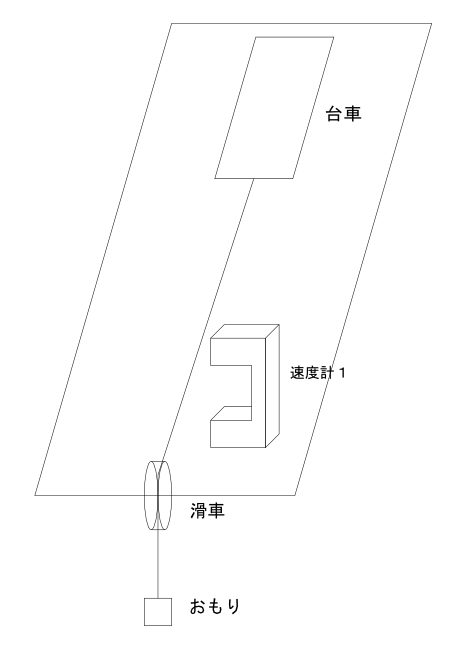
\includegraphics[scale=0.5]{zikkenzu1.png}
  \caption{実験装置配置図}    
\end{figure}
\begin{figure}[H]
  \centering
  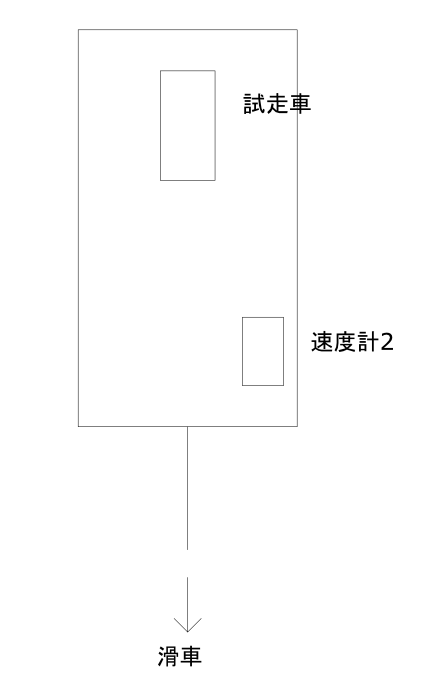
\includegraphics[scale=0.5]{zikkenzu2.png}
  \caption{台車の詳細な図}    
\end{figure}
  \begin{enumerate}
    \item 鉛直に下ろした糸の先端におもりを付け、糸を弛ませずに静かに手を離す。
    \item 台車が前方にあるストッパーにより運動を急停止させると、台車上の後方に置いてある試走車は前方に向って飛び出す。この試走車の飛び出す速度$v$を速度計2により測定する。
    \item 台車が急停止する直前の速さ$V$を速度計1で測定する。
  \end{enumerate}

\section{結果}
\begin{table}[H]
  \centering
  \caption{錘の質量$m$(kg)、台車の速度$V$(km/h)、試走車の速度$v$(km/h)}
  \begin{tabular}{|l|lll|lll|}
  \hline
  \multicolumn{1}{|c|}{錘の質量$m$(kg)} & \multicolumn{3}{c|}{台車の速度$V$(km/h)} & \multicolumn{3}{c|}{試走車の速度$v$(km/h)} \\ \hline
   & \multicolumn{1}{r|}{1回目} & \multicolumn{1}{r|}{2回目} & \multicolumn{1}{r|}{3回目} & \multicolumn{1}{r|}{1回目} & \multicolumn{1}{r|}{2回目} & \multicolumn{1}{r|}{3回目} \\ \hline
  0 & \multicolumn{1}{r|}{0} & \multicolumn{1}{r|}{0} & \multicolumn{1}{r|}{0} & \multicolumn{1}{r|}{0} & \multicolumn{1}{r|}{0} & \multicolumn{1}{r|}{0} \\ \hline
  0.01 & \multicolumn{1}{l|}{0.24} & \multicolumn{1}{l|}{0.28} & 0.25 & \multicolumn{1}{l|}{0} & \multicolumn{1}{l|}{0} & 0 \\ \hline
  0.02 & \multicolumn{1}{l|}{0.81} & \multicolumn{1}{l|}{0.82} & 0.83 & \multicolumn{1}{l|}{0} & \multicolumn{1}{l|}{0} & 0 \\ \hline
  0.03 & \multicolumn{1}{l|}{1.14} & \multicolumn{1}{l|}{1.13} & 1.13 & \multicolumn{1}{l|}{1.28} & \multicolumn{1}{l|}{1.22} & 1.24 \\ \hline
  0.04 & \multicolumn{1}{l|}{1.36} & \multicolumn{1}{l|}{1.35} & 1.37 & \multicolumn{1}{l|}{1.55} & \multicolumn{1}{l|}{1.56} & 1.55 \\ \hline
  0.05 & \multicolumn{1}{l|}{1.57} & \multicolumn{1}{l|}{1.53} & 1.59 & \multicolumn{1}{l|}{1.83} & \multicolumn{1}{l|}{1.84} & 1.87 \\ \hline
  0.06 & \multicolumn{1}{l|}{1.75} & \multicolumn{1}{l|}{1.75} & 1.75 & \multicolumn{1}{l|}{2.38} & \multicolumn{1}{l|}{2.38} & 2.38 \\ \hline
  0.07 & \multicolumn{1}{l|}{1.89} & \multicolumn{1}{l|}{1.88} & 1.89 & \multicolumn{1}{l|}{2.43} & \multicolumn{1}{l|}{2.52} & 2.52 \\ \hline
  0.08 & \multicolumn{1}{l|}{2.05} & \multicolumn{1}{l|}{2.05} & 2.05 & \multicolumn{1}{l|}{2.73} & \multicolumn{1}{l|}{2.73} & 2.73 \\ \hline
  0.09 & \multicolumn{1}{l|}{2.17} & \multicolumn{1}{l|}{2.12} & 2.16 & \multicolumn{1}{l|}{2.81} & \multicolumn{1}{l|}{2.79} & 2.85 \\ \hline
  0.1 & \multicolumn{1}{l|}{2.29} & \multicolumn{1}{l|}{2.25} & 2.3 & \multicolumn{1}{l|}{2.65} & \multicolumn{1}{l|}{2.69} & 2.82 \\ \hline
  0.11 & \multicolumn{1}{l|}{2.41} & \multicolumn{1}{l|}{2.39} & 2.41 & \multicolumn{1}{l|}{3.02} & \multicolumn{1}{l|}{3.03} & 3.01 \\ \hline
  0.12 & \multicolumn{1}{l|}{2.51} & \multicolumn{1}{l|}{2.51} & 2.51 & \multicolumn{1}{l|}{3.22} & \multicolumn{1}{l|}{3.22} & 3.22 \\ \hline
  0.13 & \multicolumn{1}{l|}{2.61} & \multicolumn{1}{l|}{2.6} & 2.61 & \multicolumn{1}{l|}{3.3} & \multicolumn{1}{l|}{3.21} & 3.32 \\ \hline
  0.14 & \multicolumn{1}{l|}{2.66} & \multicolumn{1}{l|}{2.66} & 2.66 & \multicolumn{1}{l|}{3.32} & \multicolumn{1}{l|}{3.32} & 3.22 \\ \hline
  0.15 & \multicolumn{1}{l|}{2.79} & \multicolumn{1}{l|}{2.71} & 2.78 & \multicolumn{1}{l|}{3.44} & \multicolumn{1}{l|}{3.24} & 3.11 \\ \hline
  0.16 & \multicolumn{1}{l|}{2.87} & \multicolumn{1}{l|}{2.87} & 2.87 & \multicolumn{1}{l|}{3.59} & \multicolumn{1}{l|}{3.59} & 3.59 \\ \hline
  0.17 & \multicolumn{1}{l|}{2.98} & \multicolumn{1}{l|}{2.98} & 2.99 & \multicolumn{1}{l|}{3.69} & \multicolumn{1}{l|}{3.66} & 3.58 \\ \hline
  0.18 & \multicolumn{1}{l|}{3.04} & \multicolumn{1}{l|}{3.04} & 3.04 & \multicolumn{1}{l|}{3.7} & \multicolumn{1}{l|}{3.7} & 3.7 \\ \hline
  0.19 & \multicolumn{1}{l|}{3.11} & \multicolumn{1}{l|}{3.11} & 3.1 & \multicolumn{1}{l|}{3.75} & \multicolumn{1}{l|}{3.72} & 3.65 \\ \hline
  0.2 & \multicolumn{1}{l|}{3.17} & \multicolumn{1}{l|}{3.2} & 3.18 & \multicolumn{1}{l|}{3.46} & \multicolumn{1}{l|}{3.46} & 3.59 \\ \hline
  0.21 & \multicolumn{1}{l|}{3.22} & \multicolumn{1}{l|}{3.22} & 3.25 & \multicolumn{1}{l|}{3.85} & \multicolumn{1}{l|}{3.65} & 3.71 \\ \hline
  0.22 & \multicolumn{1}{l|}{3.35} & \multicolumn{1}{l|}{3.35} & 3.35 & \multicolumn{1}{l|}{3.93} & \multicolumn{1}{l|}{3.93} & 3.93 \\ \hline
  0.23 & \multicolumn{1}{l|}{3.33} & \multicolumn{1}{l|}{3.36} & 3.38 & \multicolumn{1}{l|}{3.94} & \multicolumn{1}{l|}{4.02} & 3.97 \\ \hline
  0.24 & \multicolumn{1}{l|}{3.42} & \multicolumn{1}{l|}{3.42} & 3.42 & \multicolumn{1}{l|}{4.1} & \multicolumn{1}{l|}{4.1} & 4.1 \\ \hline
  0.25 & \multicolumn{1}{l|}{3.48} & \multicolumn{1}{l|}{3.46} & 3.89 & \multicolumn{1}{l|}{3.54} & \multicolumn{1}{l|}{3.65} & 3.52 \\ \hline
  \end{tabular}
  \end{table}
  \begin{table}[H]
    \centering
    \caption{錘の質量$m$(kg)、台車の速度$V$(km/h)の平均、試走車の速度$v$(km/h)の平均}
    \begin{tabular}{|l|l|l|}
    \hline
    錘の質量$m$(kg) & 台車の速度$V$(km/h) & 試走車の速度$v$(km/h) \\ \hline
    0    &        0 & 0\\ \hline
    0.01 & 0.256667 & 0 \\ \hline
    0.02 & 0.82 & 0 \\ \hline
    0.03 & 1.133333 & 1.246667 \\ \hline
    0.04 & 1.36 & 1.553333 \\ \hline
    0.05 & 1.563333 & 1.846667 \\ \hline
    0.06 & 1.75 & 2.38 \\ \hline
    0.07 & 1.886667 & 2.49 \\ \hline
    0.08 & 2.05 & 2.73 \\ \hline
    0.09 & 2.15 & 2.816667 \\ \hline
    0.1 & 2.28 & 2.72 \\ \hline
    0.11 & 2.403333 & 3.02 \\ \hline
    0.12 & 2.51 & 3.22 \\ \hline
    0.13 & 2.606667 & 3.276667 \\ \hline
    0.14 & 2.66 & 3.286667 \\ \hline
    0.15 & 2.76 & 3.263333 \\ \hline
    0.16 & 2.87 & 3.59 \\ \hline
    0.17 & 2.983333 & 3.643333 \\ \hline
    0.18 & 3.04 & 3.7 \\ \hline
    0.19 & 3.106667 & 3.706667 \\ \hline
    0.2 & 3.183333 & 3.503333 \\ \hline
    0.21 & 3.23 & 3.736667 \\ \hline
    0.22 & 3.35 & 3.93 \\ \hline
    0.23 & 3.356667 & 3.976667 \\ \hline
    0.24 & 3.42 & 4.1 \\ \hline
    0.25 & 3.61 & 3.57 \\ \hline
  \end{tabular}
  \end{table}
  上の台車の速度の平均と試走車の速度の平均との関係と理論値を示したのが以下図3のグラフである
  \begin{figure}[H]
    \centering
    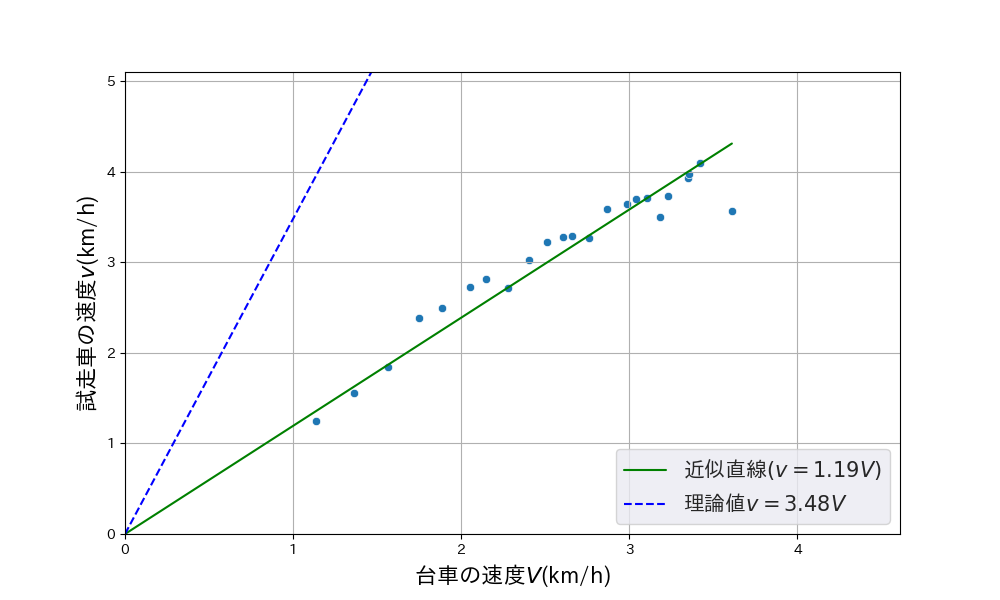
\includegraphics[scale=0.65]{Figure_2.png}
    \caption{台車の速度と試走車の速度との関係}
    \label{fig:2ji}
  \end{figure}%
  上のグラフより原理で示した予想通り試走車の速度は台車の速度に比例することがわかる。しかし、理論値である\[v=\sqrt{\frac{m_1+m_2}{m_2}}V=1.19V\]とずれが生じた。
  また、このグラフでは近似直線を導出する際に$(0.256,0),(0.820,0)$の値は省いている。なぜなら、この実験では摩擦がないものとして考えているがこの値の時は静止摩擦力により試走車が動かないため、
  実験における現象を考える上では余計な値であるからである。しかし、それ以降のデータにも摩擦の影響は出ているはずであるが、動摩擦力と静止摩擦力では物体に影響する値が異なる上に
  動摩擦力はこの場合試走車の質量に依存し一定であるため、静止摩擦力が影響している値のみを外して考えている。

  \begin{figure}[H]
    \centering
    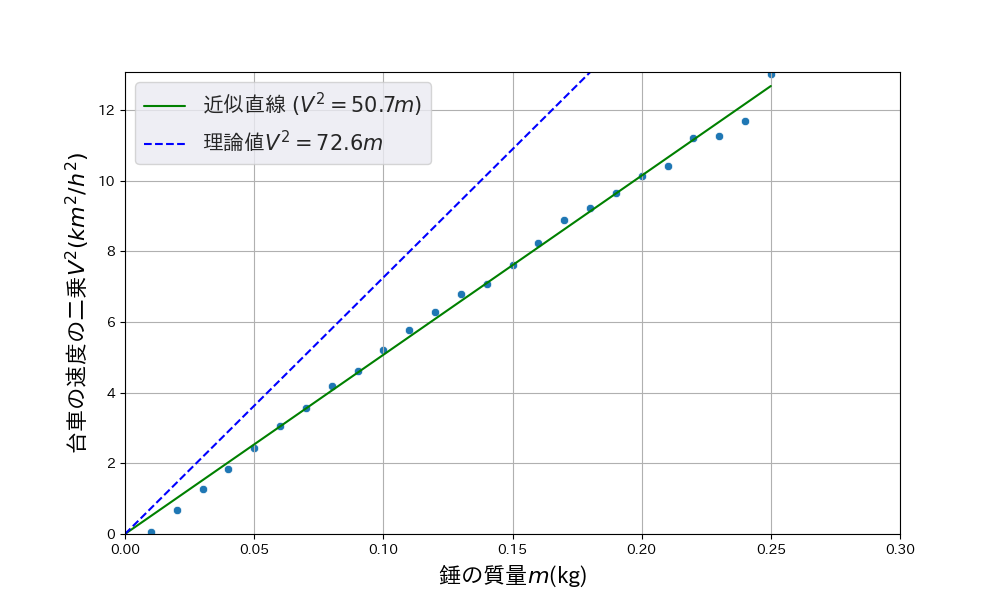
\includegraphics[scale=0.65]{Figure_3.png}
    \caption{錘の質量と台車の速度との関係}
    \label{fig:3ji}
  \end{figure}%
  上図より原理で示した予想通り台車の速度の二乗は錘の質量に比例することがわかる。しかし、理論値である\[V^2=\frac{2gL}{M}m=72.6m\]とずれが生じた。
\section{考察}
\subsection{台車の速度と試走車の速度との関係について}
結果より、理論値よりも測定値のほうが傾き、すなわち$\sqrt{\frac{m_1+m_2}{m_2}}$の値が小さいことが分かった。なぜ差が生まれたのかというとこの現象で無視していた試走車と台車との摩擦や台車と平面
との摩擦によって力学的エネルギーが損失し、台車の運動エネルギーが試走車の運動エネルギー以外にも熱や音のエネルギーとして変換されたことで試走車の速度が理論的に予測されていた速度よりも
値が小さくなったのではないかと考えられる。
\subsection{錘の質量と台車の速度との関係について}
結果より、理論値よりも測定値のほうが傾き、すなわち$\frac{2gL}{M}$の値が小さいことが分かった。その原因として考えられることは、この現象で無視していた台車と床の摩擦によって力学的エネルギーが損失し、
錘の位置エネルギーが台車の運動エネルギー以外に熱や音のエネルギーとして変換されたことで台車の速度が理論的に予測されていた速度より値が小さくなったのではないかと考えられる。
\end{document}
